\documentclass[10pt,landscape]{article}
\usepackage{multicol}
\usepackage{comment}
\usepackage{calc}
\usepackage{ifthen}
\usepackage[landscape]{geometry}
\usepackage{graphicx}
\usepackage{amsmath, amssymb, amsthm}
\usepackage{latexsym, marvosym, adjustbox}
\usepackage{pifont}
\usepackage{lscape}
\usepackage{graphicx}
\usepackage{array}
\usepackage{booktabs}
\usepackage[bottom]{footmisc}
\usepackage{tikz}
\usetikzlibrary{shapes}
\usepackage{pdfpages}
\usepackage{wrapfig}
\usepackage[shortlabels]{enumitem}
\setlist[description]{leftmargin=0pt}
\usepackage{xfrac}
\usepackage{relsize}
\usepackage{rotating}
\usetikzlibrary{positioning,shapes,arrows,matrix,bayesnet,backgrounds}
 \newcommand\independent{\protect\mathpalette{\protect\independenT}{\perp}}
    \def\independenT#1#2{\mathrel{\setbox0\hbox{$#1#2$}%
    \copy0\kern-\wd0\mkern4mu\box0}} 
            
\newcommand{\noin}{\noindent}    
\newcommand{\logit}{\textrm{logit}} 
\newcommand{\var}{\textrm{Var}}
\newcommand{\cov}{\textrm{Cov}} 
\newcommand{\corr}{\textrm{Corr}} 
\newcommand{\N}{\mathcal{N}}
\newcommand{\Bern}{\textrm{Bern}}
\newcommand{\Bin}{\textrm{Bin}}
\newcommand{\Beta}{\textrm{Beta}}
\newcommand{\Gam}{\textrm{Gamma}}
\newcommand{\Expo}{\textrm{Expo}}
\newcommand{\Pois}{\textrm{Pois}}
\newcommand{\Unif}{\textrm{Unif}}
\newcommand{\Geom}{\textrm{Geom}}
\newcommand{\NBin}{\textrm{NBin}}
\newcommand{\p}{\mathbb{P}}
\newcommand{\E}{\mathbb{E}}
\newcommand{\Hypergeometric}{\textrm{HGeom}}
\newcommand{\HGeom}{\textrm{HGeom}}
\newcommand{\Mult}{\textrm{Mult}}
\newcommand{\ind}{\perp\!\!\!\!\perp}
\newcommand{\notind}{\not\!\perp\!\!\!\perp}

\geometry{top=.2in,left=.2in,right=.2in,bottom=.2in}

\pagestyle{empty}
\makeatletter
\renewcommand{\section}{\@startsection{section}{1}{0mm}%
                                {-1ex plus -.5ex minus -.2ex}%
                                {0.5ex plus .2ex}%x
                                {\normalfont\large\bfseries}}
\renewcommand{\subsection}{\@startsection{subsection}{2}{0mm}%
                                {-1explus -.5ex minus -.2ex}%
                                {0.5ex plus .2ex}%
                                {\normalfont\normalsize\bfseries}}
\renewcommand{\subsubsection}{\@startsection{subsubsection}{3}{0mm}%
                                {-1ex plus -.5ex minus -.2ex}%
                                {1ex plus .2ex}%
                                {\normalfont\small\bfseries}}
\makeatother

\setcounter{secnumdepth}{0}

\setlength{\parindent}{0pt}
\setlength{\parskip}{0pt plus 0.5ex}

% -----------------------------------------------------------------------

\usepackage{titlesec}

\titleformat{\section}
{\color{blue}\normalfont\normalsize\bfseries}
{\color{blue}\thesection}{1em}{}
\titleformat{\subsection}
{\color{cyan}\normalfont\normalsize\bfseries}
{\color{cyan}\thesection}{1em}{}
% Comment out the above 5 lines for black and white

\begin{document}

\raggedright
\footnotesize
\begin{multicols*}{3}

	% multicol parameters
	% These lengths are set only within the two main columns
	%\setlength{\columnseprule}{0.25pt}
	\setlength{\premulticols}{1pt}
	\setlength{\postmulticols}{1pt}
	\setlength{\multicolsep}{1pt}
	\setlength{\columnsep}{2pt}

	%%%%%%%%%%%%%%%%%%%%%%%%%%%%%%%%%%%%
	%%% TITLE
	%%%%%%%%%%%%%%%%%%%%%%%%%%%%%%%%%%%%

	%%%%%%%%%%%%%%%%%%%%%%%%%%%%%%%%%%%%
	%%% ATTRIBUTIONS
	%%%%%%%%%%%%%%%%%%%%%%%%%%%%%%%%%%%%

	\section{Clustering}\smallskip \hrule height 2pt \smallskip

	$\{\mathbf{x}_n\}_{n=1}^N$ is set of points in Euclidean space.

	\subsection{K-Means}
	\begin{minipage}{\linewidth}
		\centering
	\end{minipage} \vspace{-0.25 cm}

	$\{\pmb{\mu}_k\}^K_{k=1}$ is set of cluster means. Loss is:
	\[
		\mathcal{L}(\mathbf{x}, \pmb{\mu}) = \sum_{\substack{1\leq k\leq K,\\ 1\leq n \leq n}} \mathbb{I}(k = \textrm{argmin}_j \|\mathbf{x}_n - \pmb{\mu}_j\|)\cdot \|\mathbf{x}_n - \pmb{\mu}_k\|_2^2.
	\]
	We call the indicators $r_{n,k}$.

	To optimize, randomly initialize $\pmb{\mu}_k$, then repeat:
	\begin{enumerate}
		\item Compute sets $C_k = \{ \mathbf{x}_n : k=\textrm{argmin}_j \|\mathbf{x}_n - \pmb{\mu}_j\| \}$. {\color{red} $O(NK)$}
		\item Set $\pmb{\mu}_k = \textrm{mean}(C_k)$. {\color{red} $O(N)$}
	\end{enumerate}

	\subsection{HAC}
	\begin{minipage}{\linewidth}
		\centering
	\end{minipage} \vspace{-0.25 cm}

	Define distance between sets. Greedily merge clusters. {\color{red} $O(N^3)$}
	\begin{itemize}
		\item \textbf{Min-linkage:} $d(A,B)=\min\,\{d(a,b) : a\in A, b\in B\}$.
			      {\color{red} Results in long, non-compact, sensitive-to-outlier clusters.}
		\item \textbf{Max-linkage:} $d(A,B)=\max\,\{d(a,b) : a\in A, b\in B\}$.
			      {\color{red} Results in compact, globular clusters.}
		\item \textbf{Mean-linkage:} $d(A,B)=\textrm{mean}\,\{d(a,b) : a\in A, b\in B\}$.
		\item \textbf{Centroid-linkage:} $d(A,B)=d(\textrm{mean}(A), \textrm{mean}(B))$.
			      {\color{red} Somewhere in between.}
	\end{itemize}

	\textbf{Curse of Dimensionality:} {\color{green} TODO}

	\subsection{Bayesian Mixture Models}
	\begin{minipage}{\linewidth}
		\centering
	\end{minipage} \vspace{-0.25 cm}

	Latent variables $z_n\sim \textrm{Cat}({\theta})$, $K$ categories $C_k$.
	\[
		\mathbf{x}_n \mid z_n = C_k \sim f(\mathbf{x}_n \mid \pmb{\lambda}_k)\quad\textrm{for parameters}\quad\pmb{\lambda}
	\]

	For example, $p(z_n = C_k; \theta)$ might be $\theta_k$. Goals:
	\begin{enumerate}
		\item Compute MLE for $\pmb{\lambda}$ and $\pmb{\theta}$, i.e. maximize $p(\mathbf{x}; \pmb{\lambda}, \theta)$
		\item Estimate $z_n$, i.e. maximize $p(z_n \mid \mathbf{x}_n; \pmb{\lambda}, \theta)$.
	\end{enumerate}
	Once we have (1), we have (2) by Bayes rule, however, intractible log-likelihood optimization:
	\[
		\begin{aligned}
			\log p(\mathbf{x}_n; \pmb{\lambda}, \theta)
			 & = \log \sum_{1\leq k \leq K} p(z_n = C_k; \theta)\cdot p(\mathbf{x}_n \mid z_n = C_k; \pmb{\lambda},\theta) \\
			 & = \log \sum_{1\leq k \leq K} \theta_k\cdot f(\mathbf{x}_n; \pmb{\lambda}_k).
		\end{aligned}
	\]
	\smallskip\smallskip
	\textbf{EM Algorithm}\\
	Initialize $\mathbf{\lambda}^{(0)}$, $\theta^{(0)}$ randomly. Then repeat:
	\begin{enumerate}
		\item \textbf{E-step:} Predict distribution $\textbf{q}$ for $z_n$.
		      \[q_{n,k} = p(z_n = C_k\mid \mathbf{x}_n; \pmb{\lambda}^{(t)}, \theta^{(t)}) = \frac{\theta_k \cdot f(\mathbf{x}_n \mid \pmb{\lambda}_k)}{\sum_{j=1}^K \theta_j \cdot f(\mathbf{x}_n \mid \pmb{\lambda}_j)}.\]
		\item \textbf{M-step:} Update parameters:
		      \[
			      \pmb{\lambda}^{(t+1)},\theta^{(t+1)} = \mathop{\mathrm{argmax}}\limits_{\pmb{\lambda}, \theta} \sum_{\substack{1\leq n \leq N,\\ 1\leq k \leq K}} \log (\theta_k\cdot f(x_n\mid \pmb{\lambda}_k))^{q_{n,k}}.
		      \]
	\end{enumerate}

	This algorithm is guaranteed to converge (as the likelihood weakly increases each step), but will not necessarily converge to the global optimimum.

	\[\textrm{ELBO} = \mathbb{E}_{z\sim q(z)}\log\left(\frac{p(x \mid z_n = C_k; \theta) \cdot p(z_n = C_k)}{q(z)})\right)\]

	\begin{center}
		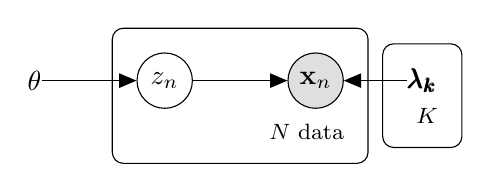
\begin{tikzpicture}
			\node[obs] (x) {$\mathbf{x}_n$};%
			\node[latent,left=of x,xshift=-0.2cm] (z) {$z_n$}; %
			\node[const,left=of z,xshift=-0.2cm] (th) {$\theta$}; %
			\node[const,right=of x,xshift=-0.2cm] (lam) {$\pmb{\lambda_k}$}; %
			% \node[latent,above=of x] (r) {$r$}; %
			% \node[latent,above=of x,xshift=1cm] (sigma) {$\sigma$}; %
			% plate
			\plate [inner sep=.3cm,xshift=.0cm,yshift=.0cm] {plate1} {(z)(x)} {$N$ data}; %
			\plate [inner sep=.3cm,xshift=.0cm,yshift=.0cm] {plate2} {(lam)} {$K$}; %
			% edges
			\edge {z} {x}
			\edge {th} {z}
			\edge {lam} {x}
		\end{tikzpicture}
	\end{center}

	\smallskip\smallskip
	\textbf{Gaussian Mixture Models}\\
	Here, $p(\mathbf{x} \mid z = C_k) = \mathcal{N}(\mathbf{x}; \pmb{\mu}_k, \pmb{\Sigma}_k)$ and $p(z_n = C_k)=\pmb{\pi}_k$. Then:
	\[
		\begin{aligned}
			\pmb{\pi}_k^{(t+1)}
			 & = \frac{1}{N}\sum_{1\leq n \leq N} q_{n,k}                                                                                                       \\
			\pmb{\mu}_k^{(t+1)}
			 & = \sum_{1\leq n \leq N} q_{n,k}\mathbf{x}_n\bigg/ \sum_{1\leq n \leq N} q_{n,k}                                                                  \\
			\pmb{\Sigma}^{(t+1)}_{k}
			 & =\sum_{1\leq n \leq N} q_{n,k}(\mathbf{x}_n - \pmb{\mu}_k^{(t+1)})(\mathbf{x}_n - \pmb{\mu}_k^{(t+1)})^\top\bigg/ \sum_{1\leq n \leq N} q_{n,k}.
		\end{aligned}
	\]

	\smallskip\smallskip
	\textbf{Topic Models}\\
	{\color{green} TODO}

	\section{Principle Component Analysis}\smallskip \hrule height 2pt \smallskip

	% \subsection{Reducing Dimensionality}
	\begin{minipage}{\linewidth}
		\centering
	\end{minipage} \vspace{-0.25 cm}

	Approximate $\mathbf{x}_n\approx \mathbf{U}\mathbf{z_n}$ where $z_n$ are lower dimensional, while minimizing reconstruction loss. If $\overline{\mathbf{x}}$ is the mean of $\mathbf{x}$, we write
	\[
		\mathcal{L}(\mathbf{z}, \mathbf{U}) = \frac{1}{N}\sum_{1\leq n \leq N}\|(x_n - \overline{\mathbf{x}}) - \mathbf{U}z_n\|^2_2,\quad\textrm{where }\mathbf{U}\textrm{ is orthogonal.}
	\]
	Minimized by matrix of biggest eigenvectors of emperical covariance matrix $\mathbf{S}=\mathbf{X}^\top \mathbf{X}/N$. Projection is $\mathbf{z} = \mathbf{U}^\top\mathbf{x}$.

	\subsection{Singular Value Decomposition Trick}
	\begin{minipage}{\linewidth}
		\centering
	\end{minipage} \vspace{-0.25 cm}

	The SVD of a matrix is $\mathbf{X} = \mathbf{UZV}^{\top}$, where $\mathbf{Z}$ is a diagonal matrix, and the columns of $\mathbf{U}$ and $\mathbf{V}$ are orthagonal ($\mathbf{V}^\top\mathbf{V} = 1$). Notice that:
	$$\mathbf{X}^{\top}\mathbf{X} = \mathbf{V} \mathbf{Z}^{\top} \mathbf{U}^{\top} \mathbf{U} \mathbf{Z} \mathbf{V}^{\top} = \mathbf{V} \mathbf{Z}^{\top}\mathbf{Z} \mathbf{V}^{\top}$$

	Sot if follows that:
	\begin{enumerate}
		\item If $\mathbf{X}$ is mean centered, then the eigenvalues of $\mathbf{S}$ can be read off as $\lambda_{k} \in \frac{1}{N} Z^{2}$

		\item The columns of $\mathbf{V}$ are the eigenvectors of the covariance matrix $\mathbf{S}$
	\end{enumerate}
	%
	\section{Bayes Nets}\smallskip \hrule height 2pt \smallskip

	\subsection{$d$-separation}
	\begin{minipage}{\linewidth}
		\centering
	\end{minipage} \vspace{-0.25 cm}

	Two sets of variables $X_A$ and $X_B$ are $d$-separated by a set of evidence $X_E$ if \emph{every} undirected path from $X_A$ to $X_B$ is ``blocked'' by $X_E$. In this case we write $X_A \perp X_B \mid X_E$.
	\begin{enumerate}
		\item $A \not \perp C$, but if $B$ observed then $\rightarrow$ $A \perp C$

		      \smallskip
		      \adjustbox{max width = 4cm}{
			      \tikz{
				      % nodes
				      \node[latent] (B) {$B$};%
				      \node[latent,above=of B,xshift=-1cm, yshift=-0.5cm] (A) {$A$}; %
				      \node[latent,above=of B,xshift=1cm, yshift=-0.5cm] (C) {$C$}; %
				      % plate
				      \plate [inner sep=.2cm,yshift=.1cm] {plate1} {(B)(A)(C)} {}; %
				      % edges
				      \edge {B} {A,C} }
			      \tikz{
				      % nodes
				      \node[obs] (B) {$B$};%
				      \node[latent,above=of B,xshift=-1cm, yshift=-0.5cm] (A) {$A$}; %
				      \node[latent,above=of B,xshift=1cm, yshift=-0.5cm] (C) {$C$}; %
				      % plate
				      \plate [inner sep=.2cm,yshift=.1cm] {plate1} {(B)(A)(C)} {}; %
				      % edges
				      \edge {B} {A,C} }
		      }

		\item $A \not\perp C$, but if  $B$ observed then $\rightarrow$ $A \perp C$

		      \smallskip
		      \adjustbox{max width = 4cm}{
			      \tikz{
				      % nodes
				      \node[latent] (B) {$B$};%
				      \node[latent,above=of B,xshift=-1cm, yshift=-0.5cm] (A) {$A$}; %
				      \node[latent,above=of B,xshift=1cm, yshift=-0.5cm] (C) {$C$}; %
				      % plate
				      \plate [inner sep=.2cm,yshift=.1cm] {plate1} {(B)(A)(C)} {}; %
				      % edges
				      \edge {A} {B};
				      \edge {B} {C} }
			      \tikz{
				      % nodes
				      \node[obs] (B) {$B$};%
				      \node[latent,above=of B,xshift=-1cm, yshift=-0.5cm] (A) {$A$}; %
				      \node[latent,above=of B,xshift=1cm, yshift=-0.5cm] (C) {$C$}; %
				      % plate
				      \plate [inner sep=.2cm,yshift=.1cm] {plate1} {(B)(A)(C)} {}; %
				      % edges
				      \edge {A} {B};
				      \edge {B} {C}}
		      }

		\item $A \perp C$ but if $B$ observed then $A \not \perp C$

		      \smallskip
		      \adjustbox{max width = 4cm}{
			      \tikz{
				      % nodes
				      \node[latent] (B) {$B$};%
				      \node[latent,above=of B,xshift=-1cm, yshift=-0.5cm] (A) {$A$}; %
				      \node[latent,above=of B,xshift=1cm, yshift=-0.5cm] (C) {$C$}; %
				      % plate
				      \plate [inner sep=.2cm,yshift=.1cm] {plate1} {(B)(A)(C)} {}; %
				      % edges
				      \edge {A} {B};
				      \edge {C} {B} }
			      \tikz{
				      % nodes
				      \node[obs] (B) {$B$};%
				      \node[latent,above=of B,xshift=-1cm, yshift=-0.5cm] (A) {$A$}; %
				      \node[latent,above=of B,xshift=1cm, yshift=-0.5cm] (C) {$C$}; %
				      % plate
				      \plate [inner sep=.2cm,yshift=.1cm] {plate1} {(B)(A)(C)} {}; %
				      % edges
				      \edge {A} {B};
				      \edge {C} {B}}
		      }
	\end{enumerate}

	\subsection{Variable Elimination}
	{\color{green} todo}

	\section{Hidden Markov Models}\smallskip \hrule height 2pt \smallskip
	%
	% \subsection{Data}
	% \begin{minipage}{\linewidth}
	% 	\centering
	% \end{minipage} \vspace{-0.25 cm}
	%
	Observations $\mathbf{x} = (x_{1}, \dots, x_{n})^{\top}$ and states (latent variables) $\mathbf{s} = (s_{1}, \dots, s_{n})^{\top}$ which follow the generative process below:

	\begin{center}
		\adjustbox{max width = 5cm}{
			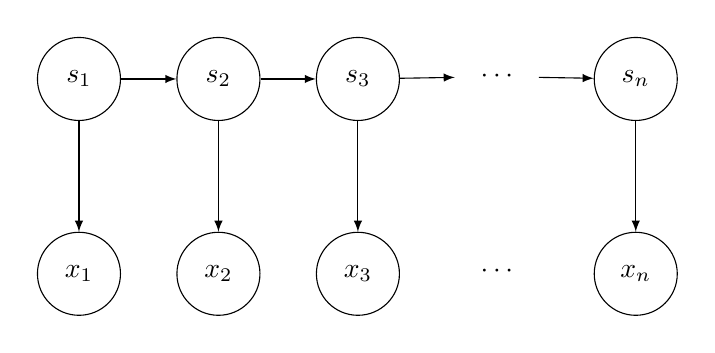
\begin{tikzpicture}
				\matrix[matrix of math nodes,column sep=2em,row
					sep=4em,cells={nodes={circle,draw,minimum width=3em,inner sep=0pt}},
					column 0/.style={nodes={rectangle,draw=none}},
					column 4/.style={nodes={rectangle,draw=none}}] (m) {
					s_1   & s_2   & s_3   & \cdots & s_{n} \\
					x_{1} & x_{2} & x_{3} & \cdots & x_{n} \\
				};
				\foreach \X in {1, 2,3,4}
					{\draw[-latex] (m-1-\X) -- (m-1-\the\numexpr\X+1) node[midway,above]{};
						\ifnum\X=4
							\draw[-latex] (m-1-5) -- (m-2-5) node[pos=0.6,left]{};
						\else
							\draw[-latex] (m-1-\X) -- (m-2-\X) node[pos=0.6,left]{};
						\fi}
			\end{tikzpicture}}
	\end{center}

	Let $P(S_1 = k)=\theta_k$, $P(s_{t+1} = i\mid s_t = j)=T_{i,j}$, and $P(x_t = m\mid s_t=k)$. The model implies that $\mathbb{P}(s_{t} \mid s_{1}, \dots, s_{t - 1}, \mathbf{x}) = \mathbb{P}(s_{t} \mid s_{t - 1}) = T_{s_{t - 1}, s_{t}}$ and $\mathbb{P}(x_{t} \mid s_{1}, \dots, s_{t}, \mathbf{x}) = \mathbb{P}(x_{t} \mid s_{t}) = \pi_{x_{t}, s_{t}}$.

	\subsection{Optimization}
	\begin{minipage}{\linewidth}
		\centering
	\end{minipage} \vspace{-0.25 cm}

	\textbf{Forward-Backwards Algorithm}\\
	We define the following

	\begin{equation*}\begin{aligned}
			\alpha_{t}(s_{t}) & = P(x_{1}, \dots, x_{t}, s_{t})
			= \pi_{x_{t}, s_{t}} \sum_{s_{t-1} \in \mathcal{C}} T_{s_{t}, s_{t - 1}} \alpha_{t - 1}(s_{t - 1})                              \\
			\beta_{t}(s_{t})  & = \p(x_{t + 1}, \dots, x_{n} \mid s_{t})                                                                    \\
			                  & = \sum_{s_{t + 1} \in \mathcal{C}} \pi_{x_{t + 1}, s_{t + 1}} \beta_{t + 1}(s_{t + 1}) T_{s_{t + 1}, s_{t}}
		\end{aligned}\end{equation*}

	Since each $\alpha_{t}$ depends on $\alpha_{t - 1}$, we can compute each $\alpha_{t}$ successively by starting at $\alpha_{0}$ in a \textit{forward pass}.
	Since each $\beta_{t}$ depends on $\beta_{t + 1}$, we can compute each $\beta_{t}$ successively by starting at $\beta_{n}$ in a \textit{backward pass}.\\
	\smallskip
	These choices are convenient because they can \textit{all} be computed in a single pass, and $\dots$ (\textit{smoothing})

	\begin{equation*}\begin{aligned}
			P(x_{1}, \dots, x_{n}, s_{t}) & = P(x_{t + 1}, \dots, x_{n} \mid s_{t}) P(x_{1}, \dots x_{t}, s_{t}) \\
			                              & = \alpha_{t}(s_{t})\beta_{t}(s_{t})
		\end{aligned}\end{equation*}
	\textbf{Expectation Maximization (EM)}\\

	We are interested in maximizing the complete date log likelihood:

	\begin{equation*}\begin{aligned}
			L(\mathbf{s}, \mathbf{x})                & = \p(s_{1} \mid \pmb{\theta}) \prod_{t = 1}^{n - 1} \p(s_{t + 1} \mid s_{t}) \prod_{t = 1}^{n} \p(x_{t} \mid s_{t})  \\
			                                         & = \theta_{s_{1}} \prod_{t = 1}^{n - 1}T_{s_{t + 1}, s_{t}} \prod_{t = 1}^{n} \pi_{x_{t}, s_{t}}                      \\
			\Rightarrow \ell(\mathbf{s}, \mathbf{x}) & = \log(\theta_{s_{1}}) + \sum_{t = 1}^{n - 1} \log(T_{s_{t + 1}, s_{t}}) + \sum_{t = 1}^{n} \log(\pi_{x_{t}, s_{t}})
		\end{aligned}\end{equation*}

	We do not have the latent ``states" $s_{t}$, so the best we can do is to maximize the expected value of the above:

	\begin{equation*}\begin{aligned}
			 & \E[\ell(\mathbf{s}, \mathbf{x})]                                                                                                                                              \\ &= \E[\log(\theta_{s_{1}})] + \sum_{t = 1}^{n - 1} \E[\log(T_{s_{t + 1}, s_{t}})] + \sum_{t = 1}^{n} \E[\log(\pi_{x_{t}, s_{t}})]\\
			 & = \sum_{k = 1}^{K} \p(s_{1} = k \mid \mathbf{x}) \theta_{k} + \sum_{t = 1}^{n - 1} \sum_{k, k' \in \mathcal{C}} \p(s_{t + 1} = k', s_{t} = k \mid \mathbf{x}) \log(T_{k', k}) \\
			 & + \sum_{t = 1}^{n} \p(s_{t} = k \mid \mathbf{x}) \log(\pi_{x_{t}, s_{t}})                                                                                                     \\
		\end{aligned}\end{equation*}

	We define $q_{t, k} = \p(s_{t} = k \mid \mathbf{x})$ and $Q_{t, t + 1, k, k'} = \p(s_{t} = k, s_{t + 1} = k' \mid \mathbf{x})$ in the equation above to give us:

	\begin{equation}\label{eq:HMMEM}\begin{aligned}
			 & \E[\ell(\mathbf{s}, \mathbf{x})]                                                                                                                                                   = \sum_{k = 1}^{K} q_{1, k} \log(\theta_{k}) + \sum_{t = 1}^{n - 1} \sum_{k, k' \in \mathcal{C}} Q_{t, t+1, k, k'} \log(T_{k', k}) \\
			 & + \sum_{t = 1}^{n} q_{t, k} \log(\pi_{x_{t}, s_{t}})                                                                                                                                                                                                                                                                  \\
		\end{aligned}\end{equation}

	We can compute $q_{t, k}$ and $Q_{t, t + 1, k, k'}$ using Bayes' rule:
	\begin{equation*}\begin{aligned}
			q_{t, k} & = \p(s_{t} = k \mid \mathbf{x})                                                                  \\
			         & = \frac{\p(x_{1}, \dots, x_{n}, s_{t} = k)}{\sum_{k = 1}^{K} \p(x_{1}, \dots, x_{n}, s_{t} = k)} \\
			         & = \frac{\alpha_{t}(k)\beta_{t}(k)}{\sum_{k = 1}^{K} \alpha_{t}(k)\beta_{t}(k)}
		\end{aligned}\end{equation*}

	\begin{equation*}\begin{aligned}
			 & \Rightarrow Q_{t, t+1, k, k'} = \p(s_{t}, s_{t + 1} \mid \mathbf{x})                                                                                                                                                                                                                       \\
			 & = \frac{\p(s_{t}, s_{t + 1}, x_{1}, \dots, x_{n})}{\sum_{s_{t + 1}} \p(s_{t}, s_{t + 1}, x_{1}, \dots, x_{n})}                                                                                                                                                                             \\
			 & = \frac{\p(x_{1}, \dots, x_{t}, s_{t}) \p(s_{t + 1} \mid s_{t}) \p(x_{t + 1} \mid s_{t + 1}) \p(x_{t + 2}, \dots, x_{n} \mid s_{t + 1})}{\sum_{s_{t + 1}} \p(x_{1}, \dots, x_{t}, s_{t}) \p(s_{t + 1} \mid s_{t}) \p(x_{t + 1} \mid s_{t + 1}) \p(x_{t + 2}, \dots, x_{n} \mid s_{t + 1})} \\
			 & = \frac{\alpha_{t}(s_{t}) T_{s_{t + 1}, s_{t}} \pi_{x_{t + 1}, s_{t + 1}} \beta_{t + 1}(s_{t + 1})}{\sum_{s_{t + 1}} \alpha_{t}(s_{t}) T_{s_{t + 1}, s_{t}} \pi_{x_{t + 1}, s_{t + 1}} \beta_{t + 1}(s_{t + 1})}
		\end{aligned}\end{equation*}

	Once we have $\mathbf{q}$ and $\mathbf{Q}$, we know all of the parameters in \ref{eq:HMMEM}, so we can solve for the MLE: $\hat{\pmb{\theta}}, \hat{\mathbf{T}}, \hat{\pmb{\pi}}$. However, since $q_{t, k}$ and $Q_{t, t + 1, k, k'}$ both depend on $\pmb{\theta}, \mathbf{T},$ and $\pmb{\pi}$, to maximize \ref{eq:HMMEM}, we need to alternate!

	\begin{enumerate}
		\item \textit{Initialize} random values for $\pmb{\theta}$, $\mathbf{T}$, and $\pmb{\pi}$
		\item Calculate $\mathbf{q}$ and $\mathbf{Q}$ holding the parameters fixed to the MLE $\hat{\pmb{\theta}}, \hat{\mathbf{T}}, \hat{\pmb{\pi}}$
		\item Holding $\mathbf{q}$ and $\mathbf{Q}$ fixed, maximize \ref{eq:HMMEM} to find the MLE $\hat{\pmb{\theta}}, \hat{\mathbf{T}}, \hat{\pmb{\pi}}$
	\end{enumerate}

	\subsection{Inference}
	\begin{minipage}{\linewidth}
		\centering
	\end{minipage} \vspace{-0.25 cm}

	Once we have estimates $\hat{\pmb{\theta}}, \hat{\mathbf{T}}, \hat{\pmb{\pi}}$, we can compute $\pmb{\alpha}$ and $\pmb{\beta}$ to do inference. Below are two examples:

	\begin{enumerate}

		\item \textbf{Prediction}
		      \begin{equation*}\begin{aligned}
				      \p(x_{t + 1} \mid x_{1}, \dots, x_{t}) & \propto \p(x_{1}, \dots, x_{t + 1})                       \\
				                                             & = \sum_{s_{t + 1}} \p(x_{1}, \dots, x_{t + 1}, s_{t + 1}) \\
				                                             & = \sum_{s_{t + 1}} \alpha_{t + 1}(s_{t + 1})
			      \end{aligned}\end{equation*}

		\item \textbf{Filtering}
		      \begin{equation*}\begin{aligned}
				      \p(s_{t} \mid x_{1}, \dots, x_{t}) & \propto \p(s_{t}, x_{1}, \dots, x_{t}) \\
				                                         & = \alpha_{t}(s_{t})
			      \end{aligned}\end{equation*}

	\end{enumerate}

	\section{Markov Decision Process}\smallskip \hrule height 2pt \smallskip

	\subsection{Model}
	\begin{minipage}{\linewidth}
		\centering
	\end{minipage} \vspace{-0.25 cm}

	\textbf{Assumptions}\\
	\begin{enumerate}
		\item $s_{t} = $ state, $a_{t} = $ action, and $r(s_{t}, a_{t}) = $ reward at time $t$. Discount future periods by $\gamma$
		\item $\pi: \mathcal{S} \to \mathcal{A}$ determines the policy we take in state $s$: $\pi(s_{t}) = a_{t}$.
		\item \textit{Markov Model}: assume stationary probabilities, and that:
		      $$\p(s_{t + 1} \mid s_{1}, \dots, s_{t}, a_{1}, \dots, a_{t}) = \p(s_{t + 1} \mid s_{t}, a_{t})$$
	\end{enumerate}

	\subsection{Optimization}
	\begin{minipage}{\linewidth}
		\centering
	\end{minipage} \vspace{-0.25 cm}

	\textbf{Value Iteration}\\

	Maximize the \textit{expected discounted value} of policy $\pi(\cdot)$ starting at $s$. Given by the \textbf{Bellman Consistency Equation:}

	\begin{equation}\label{eq:bell}V^{\pi}(s) = r(s, \pi(s)) + \gamma \E[V^{\pi}(s')]\end{equation}

	This equation implies:
	\begin{enumerate}
		\item Expected discounted value satisfies:
		      $$V^{*}(s) = r(s, \pi(s)) + \gamma \E[V^{*}(s')]$$
		\item $B(V(s)) = \max_{a}\left\{r(s, a) + \gamma \E[V(s')] \right\} = V(s)$\\
		      is satisfied $\forall s$, then $V = V^{*}$. $B(V(s))$ is the \textbf{Bellman Operator}
	\end{enumerate}

	\textit{Algorithm}

	\begin{enumerate}
		\item Initialize $V(s) = 0 \forall s$
		\item $V'(s) = \max_{a}\left\{ r(s, a) + \gamma \sum_{s' \in \mathcal{S}} \p(s' \mid s, a) V(s') \right\}$
		\item $V(s) \leftarrow V'(s) \ \forall s$
	\end{enumerate}

	\textbf{Policy Iteration}\\
	Iterates on the policy instead of the value function, using the \textit{algorithm}:

	\begin{enumerate}
		\item Initialize policy $\pi(\cdot)$
		\item $\pi'(s) = \text{argmax}_{a}\left\{ r(s, a) + \gamma \sum_{s' \in \mathcal{S}} \p(s' \mid s, a) V^{\pi}(s') \right\}$
		\item $\pi(s) \leftarrow \pi'(s) \ \forall s$
	\end{enumerate}

	\textit{Policy Evaluation}\\
	To calculate $V^{\pi}(s)$ in the equation above, we can either:

	\begin{enumerate}
		\item Solve the systems of equations implied by \ref{eq:bell} using:
		      $$\mathbf{V}^{\pi} = (\mathbf{I} - \gamma \mathbf{P}^{\pi})^{-1} \mathbf{R}^{\pi}$$
		      For $\mathbf{V} \sim |\mathcal{S}| \times 1$, $\mathbf{P}^{\pi} \sim |\mathcal{S}| \times |\mathcal{S}|$ for $\mathbf{P}^{\pi}_{s, s'} = \p(s' \mid s, \pi(s))$, and $\mathbf{R}^{\pi} \sim |\mathcal{S}| \times 1$ for $\mathbf{R}^{\pi}_{s} = r(s, \pi(s))$.

		\item Optimize by initializing $\mathbf{V}^{0}$ s.t. $\lVert V^{0} \rVert_{\infty} \in \left[0, \frac{1}{1 - \gamma} \right]$ and repeating $\mathbf{V}^{t + 1} \leftarrow \mathbf{R} + \gamma \mathbf{P}^{\pi} \mathbf{V}^{t}$ until convergence.
	\end{enumerate}

	\section{Reinforcement Learning}\smallskip \hrule height 2pt \smallskip

	\subsection{Model}
	\begin{minipage}{\linewidth}
		\centering
	\end{minipage} \vspace{-0.25 cm}

	Assumes same generative model as MDP, except stationary probabilities $\p(s_{t + 1} \mid s_{t}, a_{t})$ are unknown.\\
	\smallskip
	To infer $\p(s_{t + 1} \mid s_{t})$, need to balance \textbf{exploration} (trying new actions) and \textbf{exploitation} (doing what you think is best).

	\subsection{Optimization}
	\begin{minipage}{\linewidth}
		\centering
	\end{minipage} \vspace{-0.25 cm}

	\textbf{Value Based Methods}\\

	Goal is to find $Q^{*}$ that satisfies \textit{Bellman equation}
	$$Q^{*}(s, a) = r(s, a) + \gamma \sum_{s'} \p(s' \mid s, a) \max_{a'} Q^{*}(s', a)$$

	Balance exploitation and explortaiton using $\epsilon$-greedy policy:
	$$\pi(s) = \begin{cases} \text{argmax}_{a} Q(s, a) & \ \text{ with probability } 1 - \epsilon \\ \text{random } a \in \mathcal{A} & \ \text{ with probability } \epsilon \end{cases}$$
	Where $\epsilon \to 0$.
	$\alpha_{t}(s, a)$ is the \textit{learning rate}.\\
	\smallskip
	\textbf{SARSA}
	$$Q(s, a) \leftarrow (1 - \alpha_{t}(s, a)) Q(s, a) + \alpha_{t}(s, a)[r(s, a) + \gamma Q(s', a')]$$

	This is a weighted average of our current belief $Q(s, a)$, and a 1-step estimate $r(s, a) + \gamma Q(s', a')$. The \textbf{temporal difference} is:
	$$r(s, a) + \gamma Q(s', a') - Q(s, a)$$

	\textit{SARSA} is \textit{on-policy}, so it needs an $\epsilon$-greedy action selection to converge to $V^{*}$.\\
	\smallskip

	\textbf{Q-learning}
	$$Q(s, a) \leftarrow (1 - \alpha_{t}(s, a)) Q(s, a) + \alpha_{t}(s, a)[r(s, a) + \gamma \max_{a'}\left\{Q(s', a')\right\}] $$

	Unlike \textit{SARSA}, \textit{Q-learning} is \textit{off-policy}, so it will always converge to $V^{*}$.\\
	\smallskip
	\textbf{Convergence Conditions}\\
	\begin{enumerate}
		\item $\sum_{t} \alpha_{t} = \infty$, so we try each action a sufficient amount
		\item $\sum_{t} \alpha_{t}^{2} < \infty$, so eventually we converge
	\end{enumerate}

\end{multicols*}
\end{document}
